\documentclass{article}
\usepackage[T1]{fontenc}
\usepackage[polish]{babel}
\usepackage[utf8]{inputenc}
\usepackage{lmodern}
\usepackage{lipsum}
\usepackage{amsmath}
\usepackage{listings}
\usepackage{graphicx} 
\usepackage[margin=1in,left=1.5in,includefoot]{geometry}
\newcommand{\blank}[1]{\hspace*{#1}}
\selectlanguage{polish}
\author{Michal Kolendo}
% header and footer stuff
\usepackage{fancyhdr}
\pagestyle{fancy}
\fancyhead{}
\fancyfoot{}
\fancyfoot[R]{\thepage\\}
\renewcommand{\headrulewidth}{0pt}
\renewcommand{\footrulewidth}{1pt}
%
 
\begin{document}
 
\begin{titlepage}
\begin{center}
\line(1,0){400}\\
[0.25in]
\huge{\bfseries Sprawozdanie}\\
[2mm]
\line(1,0){300}\\
[1.5cm]
\textsc{\LARGE Problem Generowania Stołówki}\\
[0.75cm]
\textsc{\Large Algorytmy i Struktury Danych}\\
[10cm]
\vspace{-9cm}
\textsc{Java}\\
[1cm]
\vspace{9cm}
\end{center}
\begin{flushright}
\textsc{\large Michał Kolendo\\
\small Nr indeksu 286771  \\
\large 26 Styczeń, 2017}
\textsc{\large Bartek Królak\\
\small Nr indeksu 284922  \\
\large 26 Styczeń, 2018}
\end{flushright}
\end{titlepage}
% Front matter stuff
\pagenumbering{arabic}
 
 
 
%this is main body stuff
\setcounter{page}{1}
\section{\underline{Diagram Klas}}
		\begin{figure}[h]
		\hspace*{-5.3cm} 
				\includegraphics[width=1.4\textwidth]{Diagram Klas.png}
				\caption[Diagram Klas programu Time2Dine] {{\sl Diagram Klas programu Time2Dine}}
				\label{Diagram Klas programu Time2Dine}
		\end{figure}
Z powodu wielkości diagramu obejmującego cały projekt wraz z metodami oraz polami, został on zamieszczony w załączniku do projektu pod nazwą \verb|Pełny Diagram UML programu Eggcelent|


\newpage
\section{\underline{Opis zmian w klasach}}

\begin{center}
\vspace{3mm}
\underline{\huge\textbf{{Pakiet Model}}}
\end{center}
\subsection{Chromosome}
\indent Moduł \verb|Chromosome| uległ srednim zmianom.
Zrezygnowaliśmy z przechowywania informacji binarnej na temat rozłożenia mebli w Chromosomie, gdyż została zmieniona metoda mutacji oraz krzyżowania się chromosomów ze sobą. Funkcję generowania chromosomu z \verb|Algorithm| przenieśliśmy również do klasy \verb|Chromosome|.
\begin{center}
\vspace{3mm}
\underline{\huge\textbf{{Pakiet Count}}}
\end{center}
\subsection{Algorithm}
\indent W tej klasie zrezygnowaliśmy z funkcji \verb|generateChromosome(Canteen canteen)| na rzecz klasy \verb|Chromosome|. \\Argumentami funkcji krzyżującej oraz mutującej Chromosom stała się \verb|ArrayList<Chromosome> chromosomes|.
\subsection{INAlgorithm}
\indent Zaplanowane przez nasPrototypy funkcji \verb|void mutate(ArrayList<Chromosome> chromosomes)| oraz \verb|chromosome crossBreed(ArrayList<Chromosome> chromosomes)| zmieniły argument jaki przyjmują. W funkcji krzyżującej postanowiliśmy zwracać chromosom powstały z krzyżowania i mutacji.
\begin{center}
\vspace{3mm}
\underline{\huge\textbf{{Nowe Klasy}}}
\end{center}
\subsection{FurnitureEnum}
\indent Zdecydowaliśmy się na stworzenie klasy \verb|Enum| ,która będzie przechowowyała informacje o tym jakiego rodzaju jest mebel. Stworzyliśmy w niej funkcje \verb|getWidth(FurnitureEnum furEnum)| oraz \verb|getHeight(FurnitureEnum furEnum)| zwracające kolejno szerokość i wysokość obrazka poszczególnego mebla.
\subsection{Model}
\indent Została stworzona klasa \verb|Model| usprawniająca wspomaganie realizacji funkcji programu poprzez podmetody:\\
\indent \verb|Canteen createCanteen(double bWall, double tWall, double rWall, double lWall)|\\
\indent \verb|ArrayList<Chromosomes> createPopulation(Canteen canteen)| \\
\indent \verb|ArrayList<Chromosomes> nextGeneration(Canteen canteen, ArrayList<Chromosomes> chromosomes)|\\
\newpage
\subsection{Controller}
\vspace{1mm}
\indent Został stworzony Controller zarządzający całym przebiegiem programu, przetwarzających najważniejsze dane algorytmu:\\
\verb|Chromosome getBestChromosome()| -- pobranie najlepiej przystosowanie chromosomu z populacji\\
\verb|double getIterNumber()| -- pobranie numeru iteracji programu.\\
\verb|void nextGeneration()| -- przejście do kolejnej generacji chromosomów.\\
\verb|void setCanteenCosts(FurnitureEnum key, int cost)| -- ustawienie ceny danego rodzaju mebla\\
\verb|void setAlgorithmSettings(String key, int cost)| -- ustawienie informacji o współczynnikach algorytmu\\

\begin{center}
\vspace{3mm}
\underline{\huge\textbf{{Pakiet ComponentsImage}}}
\end{center}
\indent W tym pakiecie zgodnie z założeniem znalazły się zdjęcia mebli używanych przy projekcji stołówki. Zostały one odpowiednio wyskalowane oraz poddane lekkim zmianom w programie \verb|GIMP|.
\section{\textbf{\underline{Opis algorytmu}}}

\indent  Założenia dotyczące algorytmu genetycznego zostały przez nas zmienione. Zrezygnowaliśmy z reprezentacji bitowej stołówki, gdyż musieliśmy zmierzyć się z problemem nieregularnego rozłożenia rodzajów mebli z Chromosome, przez co obligatoryjnym byłoby ustalenie poprawnej długości ciągu bitów reprezentujących odpowiednio: krzesła, stoły,ławy,drzwi,okna oraz resztę wyposażenie. Mutacja zachodzi poprzez zmiane mebla na jego inny odpowiednik. Stół cztero-osobowy zostaje zamieniony na sześcio-osobowy, mała lawa na dużą ławę oraz analogicznie inne rodzaje mebli. Krzyżowanie polega na znajdywaniu w dwóch chromosomach tych samych mebli oraz wyznaczenie nowej pozycji dla tego mebla na podstawie pozycji jego rodziców.\\
\begin{center}
\underline{Funkcja Ewaluacji}
\end{center}
\indent Pisząć funkcji ewaluacji, zdecydowaliśmy się na zliczanie pojedynczych rodzaji mebli oraz odpowiednie ich punktowanie, w zależności od przedziału w jakim się znajdują. Stołówka z duża liczbą lamp miała dużo niższą punktację niż stołówka z różnymi rodzajami mebli.W celu zrandomizowania wygenerowywanych stołówek, zrezygnowaliśmy z badania odległości między meblami.
\newpage
\section{\underline{Testy programu}}
\indent Zostało stworzonych kilka testów klasy \verb|Canteen| przy użyciu nowej Biblioteki \verb|Spock|. Ich wynik znajduje się poniżej:
\subsection{Testy jednostkowe}
\indent Do wykonania testów jednostkowych została wykorzystana biblioteka \verb|Spock|. 
Zdjęcia z wykonania testów:\\
\vspace{1cm}
\begin{figure}[h]
		\hspace*{2.7cm} 
			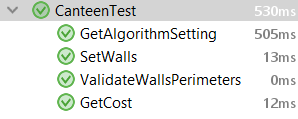
\includegraphics[width=0.5\textwidth]{CanteenTest.png}
				\caption[Testy jednostkowe] {{\sl Testy jednostkowe}}
				
		\end{figure}
\newpage

\subsection{Testy całościowe}
\indent Testy całościowe zostały przeprowadzone na interfejsie graficznym zaimplementowanym przez nas, przy próbie projekci stołówki.\\
 Przykład testu całościowego dla stołówki o parametrach \verb|10m, 10m, 8m,8m|:
\vspace{1cm}

\begin{figure}[h]
\hspace*{-1.5cm} 

\includegraphics[width=1.2\textwidth]{TestCalosciowyGen.png}
\caption[Test Całościowy] {{\sl Test Całościowy}}
\end{figure}
\section{\underline{Przykładowe użycie programu}}
\indent Zaprezentowane zostaną tu dwie przykładowe stołówki wygenerowane przez nasz algorytm genetyczny.
\begin{enumerate}
	\item Najlepsza stołówka dla pierwszej populacji:
\begin{figure}[h]
\hspace*{-2.8cm} 

\includegraphics[width=0.4\textwidth]{stolowka1.png}
\end{figure}
\newpage
\item Najlepsza stołówka dla dziesiątej populacji:
\begin{figure}[h]
\hspace*{2.4cm} 

\includegraphics[width=0.2\textwidth]{stolowka2.png}
\end{figure}

\end{enumerate}
\section{Kompilacja}
Program jest przeznaczony na dowolony system operacyjny. Ze wzglęgu na to ,iż wirtualna maszyna Java zajmuję się kompilacją programu, a nie system operacyjny na którym program jest, możemy używać Generatora stołówek gdziekolwiek. Wystarczy stworzyć odpowiedni plik \verb |.jar| projektu. 

\section{Podsumowanie}
Większość rzeczy przewidzianych przez nas w \verb|Specyfikacja Implementacyjna Time2Dine| zostało doprowadzonych do skutku. Program działa w dużej mierze tak jak powinien. Gdybyśmy mieli więcej czasu na ulepszenie projektu, moglibyśmy poprawić kwestie kosmetyczne oraz zrefaktoryzować związek klasy \verb|Controller| z klasą \verb|GUI|,
\end{document}
